\documentclass[12pt]{article}
\usepackage{url}
\usepackage{fullpage}
\usepackage{graphicx}

\begin{document}

\title{Deep Learning Movie Recommendations}
\author{Jeffrey Lund}
\date{}
\maketitle

\begin{abstract}
Recommendation systems are an important part of movie streaming services like
Netflix.
I propose a deep learning approach based on autoencoders to produce a
collaborative filtering system which predicts movie ratings for a particular
user based on a large database of ratings from other users.
My system outperforms a user-based neighborhood baseline both in terms of mean
squared error on predicted ratings and in a survey in which users judge
between recommendations from both systems.
\end{abstract}

\section{Introduction}
\label{sec:intro}

Movie streaming services like Netflix, Hulu, Amazon Prime, and
others are increasingly used by consumers to enjoy video content.
For example, in 2017 Netflix subscribers collectively watched more than 140
million hours per day and Netflix is on track to exceed \$11 billion in revenue
this year.
Undoubtedly, movie streaming services have become an integral
part of how we consume video content today.

For movie streaming services like Netflix, recommendation systems are
important for helping users to discover new content to enjoy.
In fact, roughly 80\% of hours streamed on Netflix were influenced by their
proprietary recommendation system~\cite{netflix}.
While the details of this system are mostly confidential, what we do know is
that it is a combination of various individual recommendation systems,
including some systems which leverage collaborative filtering systems.
With this in mind, the problem I examine is movie recommendations through
collaborative filtering.

In the context of movie recommendation, collaborative filtering aims to predict
unknown movie ratings for a particular user, based on that user's known ratings
as well as the movie ratings by other users in the system.
The underlying assumption is that if we can accurately predict movie ratings,
then we can recommend new movies to users that they are
likely to enjoy, including films the user may not have considered before.

The most popular approaches for collaborative filtering are discussed in
Section~\ref{sec:related}.
These methods work by computing neighborhoods of similar users or items.
In contrast, in Section~\ref{sec:arch} I propose a deep learning approach for
collaborative filtering based on an autoencoder.
I demonstrate in Section~\ref{sec:results} that my approach outperforms
the neighborhood-based baseline.

\section{Related Work}
\label{sec:related}

The most common method of performing collaborative filtering is to utilize a
k-nearest-neighbor approach between users~\cite{user-user}.
With this technique, we first start with a user-item matrix $R$, where
$R_{i,j}$ gives the rating of user $i$ for item $j$.
Typically the value $0$ indicates that a particular rating is missing.
From $R$ we then compute a user-user similarity matrix $S$, where $S_{i,j}$
gives the similarity between user $i$ and user $j$.
Naively this can be computed with $R \cdot R^T$, although using other distance
metrics such as the correlation similarity measure or cosine similarity to
population $S$ are also effective.
Once we have computed $S$, we can then predict the rating of user $i$ for item
$j$ by computing ${R^T}_k \cdot S_i$, which essentially computes the average of
the other users' ratings for item $j$ weighted by their similarity to user $i$.

Alternatively, we can use the $k$ most similar users to user $i$ to predict
the rating for item $j$.
Empirically, this seems to work better than the weighted average over all
users, although some extra work is required at test time in order to compute
the $k$ nearest neighbors.
This approach relies on the assumption that two users rated the same item
similarly, they are likely to rate other items similarly as well.
At scale, data structures such as ball trees~\cite{ball-tree} and k-d trees (a
binary space partition tree in k-dimensions) have been utilized to more
efficiently compute local neighbors between user profiles.

An alternative k-nearest-neighbor approach instead computes similarity between
pairs of items (as opposed to users) with the idea that users who like a
particular item will like similar items~\cite{item-item}.
With this approach we compute an item to item similarity matrix $I$ as $R^T R$.
As before, we can also use other similarly metrics to populate $I$.
In order to predict the rating for user $i$ on item $j$ we then compute $R_i
\cdot I_j$, which gives an average of the ratings given by user $i$ weighted by
the similarity of those items to item $j$.
Since there tends to be many more users than items in a recommendation system,
user-user collaborative filtering can be much more performant, although my
preliminary experiments with movie ratings indicate that user-user produced
more accurate predictions of movie ratings.

Another common method for performing collaborative filtering is with matrix
factorization~\cite{matrix-factorization}.
With this technique a user-item matrix is factorized into two matrices with the
inner dimension representing some latent factors using techniques such as
singular value decomposition.
The resulting factorization represents both users and items in terms of the
latent factors in such a way that they can be used to recommend new items.
As with item-item neighborhood approaches, my preliminary experiments on movie
ratings indicate that user-user neighborhood approaches are superior to matrix
factorization.

Deep learning has revolutionized many fields of computer science, including
natural language processing~\cite{deep-survey}.
Despite this, deep learning is relatively new in the area of recommendation
systems, and has not received much attention~\cite{dl-recsys-survey}.
The aim of this project is to experiment with deep learning for collaborative
filtering on a large set of movie ratings.

\section{Preliminaries}

Before I proceed with describing my exact approach, there is some value in
understanding the dataset and experimental setup that I take in this project.
I first describe the MovieLens dataset that I experiment with, and then
briefly explain the baseline model I use as a point of comparison.

\subsection{MovieLens Data}

In academia the most well known movie ratings dataset is undoubtedly the
MovieLens dataset~\cite{movielens},
although a close second is probably the Netflix prize data released via
Kaggle\footnote{https://www.kaggle.com/netflix-inc/netflix-prize-data}.
For my project, I utilize the latest version of the MovieLens
dataset, which is the recommended version for education and
development\footnote{https://grouplens.org/datasets/movielens/latest}.
This data is provided by GroupLens, which is a social computing research lab
at the University of Minnesota.

\begin{figure}
\centering
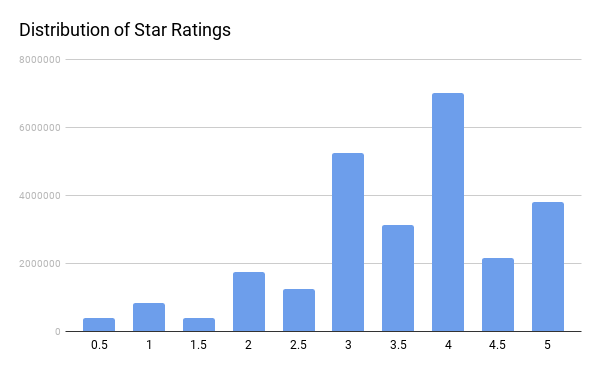
\includegraphics[width=.5\textwidth]{stars}
\caption{Distribution of ratings in the full MovieLens dataset.}
\label{fig:stars}
\end{figure}

The full MovieLens dataset contains ratings for 45,115 movies provided by
270,896 different users.
In total, the dataset contains 26,024,289 individual movie ratings.
Each rating allows users to assign between half a star and five stars to a
film, in half star increments.
Figure~\ref{fig:stars} shows the distribution of the ratings in the data.

Each rating is also accompanied by a time stamp.
Because the dataset does not contain a standard train/test split,
I used these time stamps to split the data into training and test sets, with
the oldest 90\% of the data making the training set and the newest 10\% of the
data composing the test set.
I did this with the intent to mimic the problem faced by real world movie
recommendation systems which have all of the data up to a certain point in
time, and are faced with predicting movie ratings going forward in time.

\subsection{Baseline}

As previously mentioned in Section~\ref{sec:intro}, there are a number of
popular methods for performing collaborative filtering,
including nearest-neighbor based technique comparing user-user
similarity~\cite{user-user},
nearest-neighborhood comparing item-item similarity~\cite{item-item},
and matrix factorization techniques~\cite{matrix-factorization}.
Due to limits on my computational resources, I did not have the time to use
them all on the full MovieLens dataset, especially if one considers the
various hyperparameters such as the size of the neighborhoods.

Specifically, I do not have enough RAM to fully vectorize these
algorithms.
For example, the vectorized version of the user-user nearest neighbor approach
would require computing a user-user similarity matrix which takes nearly 600 GB
in RAM%
\footnote{I could of course use a sparse matrix, but any time two users have
even a single overlapping movie there will be a non-zero entry in the
user-user matrix. So even sparse storage results in a matrix which cannot be
computed without significant thrashing.}.
The non-vectorized brute force version of the algorithm required more than a
week to finish.

In order to determine which baseline I should use on the full dataset, I
utilized a small version of the MovieLens dataset which contained only 943
users and 1,682 movies as a development dataset.
Once again I split this data into a train/test split, and measured the mean
squared error of the predictions of each of the proposed baseline algorithms.
Without going into too much detail, I determined user-user neighborhood
approach with cosine similarity and a neighborhood size of 5 performs the best
with respect to mean squared prediction error.
Consequently, this is the algorithm I utilize as my sole baseline on
the full MovieLens dataset.

\section{Model Architecture}
\label{sec:arch}

Now that we understand the MovieLens dataset and baseline methods, I will
describe the deep learning architecture I propose as an alternative to the
user based neighborhood approach.
The first thing I consider is the dimensions of the input and output of the
neural network.
In order to maximize the amount of training data I can feed to the network, I
will consider a training example to be a user profile (i.e. a row from the
user-item matrix $R$) with one rating withheld.
The loss of the network on that training example must be computed with respect
to the single withheld rating.
The consequence of this is that each individual rating in the training set
corresponds to a training example, rather than each user.

Because I am interested in what is essentially a regression, I choose to use
mean squared error with respect to known ratings as my loss function.
Compared to the mean absolute error, mean squared error more heavily penalizes
predictions which are further off.
I reason that this is good in the context of recommendation system because
predicting a high rating for an item the user did not enjoy significantly
impacts the quality of the recommendations.
On the other hand, smaller errors in prediction will likely result in
recommendations that are still useful - perhaps the regression is not
exactly correct, but at least the things with the highest predicted rating are
likely to be relevant to the user.

Initially, my architecture consisted of input from the row of the user-item
matrix $R$ with the rating for some item $j$ withheld, along with a one-hot
encoded query which indicated the network should predict the rating for user
$i$ on item $j$.
Unfortunately, this architecture proved difficult to train, probably because
the network must learn to understand not only user profiles, but also the
interplay between those profiles and the query inputs.
With respect to the mean squared error on the training data, I never achieved
a loss less than around 1.2 with this architecture.

\begin{figure}
\centering
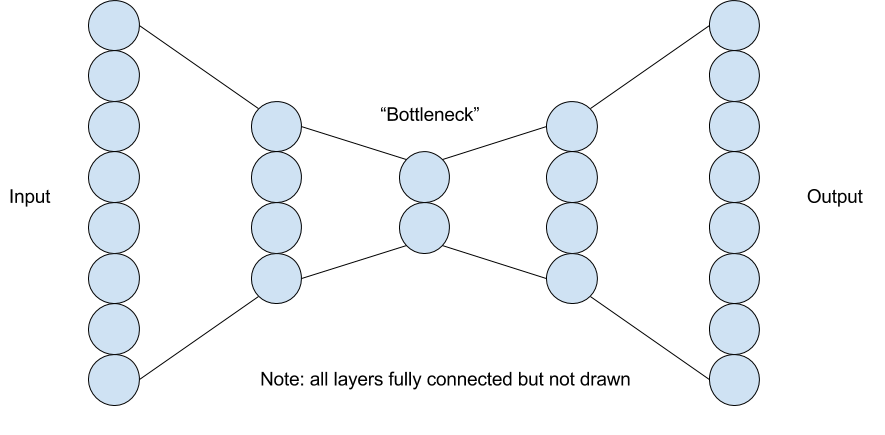
\includegraphics[width=.5\textwidth]{arch}
\caption{Overview of my network architecture.}
\label{fig:arch}
\end{figure}

Instead, I take inspiration from the concept of an autoencoder to design my
neural architecture (see Figure~\ref{fig:arch}).
This simple architecture takes an input and connects it to some number of fully
connected hidden layers which include a ``bottleneck''.
This bottleneck is a hidden layer which has a much smaller dimensionality than the
input.
The output of the network is then re-expanded to have the same dimensionality
as the input.
The network is then trained to learn the identity function, with the idea that
in order for the network to compute the identity function through the
bottleneck, it must learn a dense representation of the input.
Therefore, the autoencoder could be viewed as something akin to a
dimensionality reduction technique.
We can also hope that the bottleneck layer learns something useful related to
the structure underlying the input.
For example, a particular neuron in the bottleneck layer might represent
something related to the genre of a movie or similar movie groupings.

Ultimately though, I am not interested in learning to compute an identity
function - after all, my goal is to predict \textit{missing} ratings, not
reproduce the zeros in the input vectors.
Consequently, while my final network architecture resembles an autoencoder with
the bottleneck hidden layers and the matching dimensions on input and output,
my network is actually trained using a loss function for regression
(specifically mean squared error)
with the aim of learning to predict missing ratings.

More specifically, the training examples to the network are user
profiles with one rating withheld, and the output is the predicted ratings for
\textit{all} movies in the dataset.
While the network is expected to predict ratings for every movie based on a
user profile, I only have the answer for the one withheld rating.
Consequently, I only propagate loss for the single missing rating when
learning from the training example%
\footnote{In code, this can be accomplished with the $tf.gather$ function.}

This does have the unfortunate consequence that my model will only be able to
learn ratings for things similar to what the user has actually watched, as the
loss function is not directly affected way by the output on unrelated movies.
Due to the bottleneck layer, the model will have to generalize to some degree,
but the model may have difficulty for items which are drastically different
than the things the user actually rated.
While users do watch things they rate lowly, most of the time they do not rate
more than a few hundred items, and avoid watching completely irrelevant items,
so it may difficult for the model to predict ratings for completely unrelated
items.

For the purposes of my loss function, which is mean squared error on known
ratings, the fact that my network may not learn how to output ratings for
completely unrelated films does not seem to affect the test loss, probably
because the films in the test data are related enough that the patterns
learned from the training data generalize to the ratings in the test data.
Of course, it may affect the rankings, so it could be desirable to add a
regularization term to the loss which encourages sparsity in the output%
\footnote{To be clear, I did \textit{not} implement this regularization,
although given more time I would experiment with this.}.

With this basic design in place, I experimented with several variations of
this architecture using various numbers of layers, and various sizes for the
bottleneck layer.
The most interesting parameter was the size of the smallest bottleneck layer,
and after experimenting with various values,  eventually settled on a
bottleneck size of $512$.
From there I experimented with different numbers of fully connected layers,
always using powers of $2$ to increase and decrease the dimensionality.
The network topology I finally settled on had 7 fully connected hidden layers,
with the dimensions
$[4096, 2048, 1024, 512, 1024, 2048, 4096]$.
Each layer used a rectified linear unit%
\footnote{The rectified linear unit, or ReLU, is defined as $max(0, x)$. While
simple, it is currently the state-of-the-art in activation functions for deep
neural networks.}
as the non-linear activation function.
The connecting weights of the hidden layers were initialized using Xavier
initialization~\cite{xavier}, and the biases were initialized to zeros.

\section{Results}
\label{sec:results}

\begin{figure}
\centering
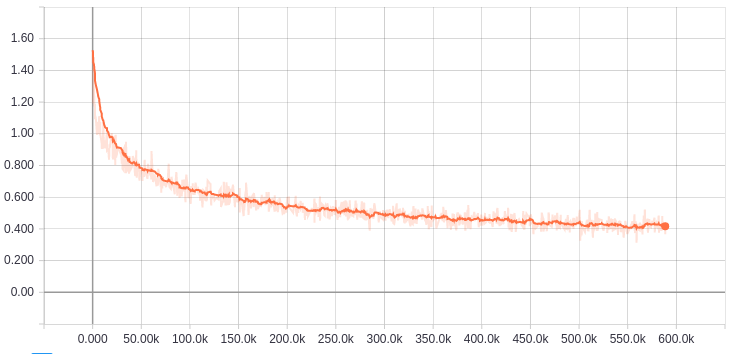
\includegraphics[width=.5\textwidth]{train}
\caption{Graph showing loss (mean squared error) decreasing over time. Each
step represents 1000 training examples.}
\label{fig:train}
\end{figure}

Using 90\% of the full MovieLens dataset as training, I trained the
architecture described in Section~\ref{sec:arch}.
It took roughly 4 days using a Titan X GPU to make 30 passes over the entire
data before the training loss stabilized.
Figure~\ref{fig:train} shows the training loss (i.e. mean squared error)
decreasing over time.
I now discuss the results of that model on the test set and compare those
results to my user based neighborhood baseline.

\subsection{Mean Squared Error}

\begin{table}
\centering
\begin{tabular}{|l|l|l|}
\hline
& User-User KNN & Model-based\\\hline
Train & N$\backslash$A & 0.4209\\\hline
Test & 11.6715 & 2.4844\\\hline
\end{tabular}
\caption{Mean squared error for my user-based neighborhood baseline, and
autoencoder inspired model-based approach.}
\label{tab:mse}
\end{table}

Table~\ref{tab:mse} summarizes the results comparing my model-based approach
with the user-based neighborhood baseline.
On the training data, my approach is stabilized around 0.42.
The neighborhood approach has learned parameters, as it simply relies on the
training data itself to make predictions.
Consequently, there is no training loss to report.

On test data, my algorithm outperforms the neighborhood approach by a large
margin.
However, it should be noted that for the purpose of making movie
recommendations, we do not actually care about the error.
Instead what we care about is the ranking of the top few most highly rated
movies.
It is not an unreasonable assumption that the algorithm which ranks
better will also have lower mean squared error,
but it is entirely possible that despite the higher errors, the top ranked
movies from the baseline approach produce superior recommendations.
This is especially true when you consider that my algorithm does not directly
learn about highly unrelated movies.

\subsection{User Evaluation}

In order to establish the usefulness of my collaborative filtering approach
when applied to movie recommendations, I performed a small user study in which
users had the chance evaluate movie recommendations made by both my system and
the baseline system.

\begin{figure}
\centering
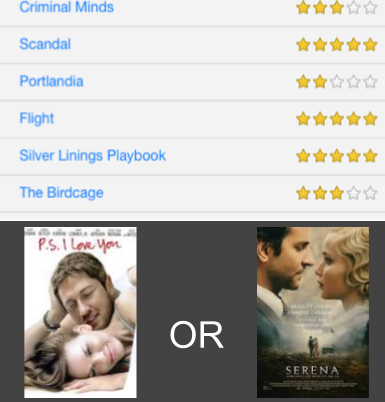
\includegraphics[width=.5\textwidth]{user}
\caption{An example of the type of questions users were asked to answer in the
user evaluation of my model-based system and the user-based neighborhood
approach.}
\end{figure}

Users were shown a user profile, which consisted of every movie a particular user
had rated, as well as the associated ratings.
The user was then presented two possible recommendations: one from my system
and one from the baseline approach.
The recommendations were chosen by picking the movie with the highest predicted
rating from either system, excluding movies that had already been rated by the
user.
The order in which the two possible recommendations were shown was randomized.
Users were asked to pick which recommendation they thought was more relevant
to the given user profile.

A total of 8 participants were used in the study.
Each user was asked to rate 15 randomly chosen recommendations.
In this survey, 71.67\% of the time users preferred the recommendation made
using my deep learning approach over the recommendation made by the baseline
approach.

While this result is encouraging, in the interest of scientific honesty, I
should be clear that this survey has a number of problems.
In addition to being an extremely small sample size,
the participants self-volunteered after I posted a link to a video
game related discord server.
I am unsure what the result of this bias will be, but am sure that sampling
from my friends is not a sound sampling strategy.

Another issue with this survey was the fact that all 8 participants indicated
to me that they were unfamiliar with most of films referenced in the survey.
The directions of the survey indicate that they were allowed to uses resources
like Google and IMDB while making their judgements, but ultimately, the
quality of these determinations must be called into question due to the lack
of familiarity.

The best user evaluation would be to actually observe the behavior of the
user of the recommendation system.
This type of click data is likely the signal used by companies such as Netflix
to measure the performance of their recommendation system.
Obviously, I do not have access to this type of resource and so for the
purposes of this project will make due with this flawed user study.

\subsection{Clustering}

The final idea that I experimented with was the idea of using the smallest
bottleneck layer in the network as something of a natural clustering.
By forcing the input into such a small dimensional space, the model must
necessarily learn something about the underlying structure of the input data.

My hypothesis was that by fixing a single neuron in the bottle neck layer and
zeroing out the remaining neurons in the bottleneck layer, and then optimizing
the input space for this particular activation, I could visualize that
structure by showing the films which trigger each cluster.
For example, I expected that there might be a neuron or small set of neurons
which trigger for various genres of film, or various styles of filmography.

\begin{table}
\centering
\begin{tabular}{|l|}
\hline
Jules and Jim (Jules et Jim) (1961)\\
Frankenstein Must Be Destroyed (1969)\\
Lolita (1962)\\
Lawnmower Man, The (1992)\\
First Knight (1995)\\
Urban Legends: Final Cut (2000)\\
Fair Game (1995)\\
Guinevere (1999)\\
Paradine Case, The (1947)\\
400 Blows, The (Les quatre cents coups) (1959)\\
\hline
\end{tabular}
\caption{Example of a ``cluster'' when optimizing the input to trigger a single
bottleneck neuron.}
\label{tab:cluster}
\end{table}

Unfortunately, this turned out not to be the case.
Table~\ref{tab:cluster} gives an example of such a ``cluster'' from optimizing
the input to trigger a single bottleneck neuron.
These movies do not seem to have any common theme, nor was there any
discernible theme to any other such cluster.

Obviously for this network to be able to accurately predict movie ratings it
must learn some sort of structure.
Evidently, this structure is far more distributed throughout the bottleneck
layer than I hypothesized.
One potential solution to this problem could be to add a regularization term
to the loss which encourages sparsity in the bottleneck layer.
However, due to time constraints, I was unable to implement this improvement.

\section{Conclusion}

Overall, I have proposed a simple neural model which performs well in terms of
mean squared error for collaborative filtering.
This adds to existing literature which suggests that deep learning can be a
powerful tool for a variety of problems in information
retrieval~\cite{dl-recsys-survey}.

In the end, this work still needs some amount of improvement before it can be
considered worthy of publication, particularly on the subject of user
evaluation.
Additional experimentation with regularization would also be merited.
That said, this system was able to handily outperform the neighborhood-based
baseline, and was able to provide superior movie recommendations.

As an added advantage of this approach, it is much more scalable at test time.

\bibliographystyle{plain}
\bibliography{report}

\end{document}
